\documentclass[11pt,a4paper]{article}

\usepackage[margin=1in]{geometry}
\usepackage{graphicx}
\graphicspath{{images/}}
\usepackage[hidelinks]{hyperref}
\usepackage{enumitem}
\usepackage{amsmath}
\usepackage{float}
\usepackage{booktabs}
\usepackage{setspace}
\usepackage{caption}
\usepackage{titlesec}
\usepackage{microtype}
\usepackage{newtxtext,newtxmath}

\setstretch{1.08}
\captionsetup{font=small}
\titlespacing{\section}{0pt}{0pt}{10pt}
\titlespacing{\subsection}{0pt}{8pt}{4pt}
\raggedbottom
\setlength{\parindent}{0pt}
\setlength{\parskip}{0.55em}
\urlstyle{same}

\begin{document}

%----------------------------------
\begin{center}
{\Huge\bfseries Late Antiquity Modeling Project\par}
\vspace{1.1em}
{\Large Visibility-Coupled Path Inference and Evaluation in Archaeological Landscapes\par}
\end{center}

\vspace{1.6em}
\section*{Personal Details}

\textbf{Name:} Ujjwal Singh

\textbf{Email:} \href{mailto:ujjosing@gmail.com}{ujjosing@gmail.com}

\textbf{GitHub:} \url{https://github.com/fallofpheonix}

\textbf{Organization:} The Late Antiquity Modeling Project

\textbf{Project idea:} Make visibility a tested and measurable part of the LAMP movement pipeline.

\clearpage

%----------------------------------
\section*{Technical Knowledge}

I have experience building reproducible Python pipelines for raster data, simulation, and spatial analysis. I am comfortable with NumPy, Rasterio, GDAL-based workflows, CRS handling, raster alignment, and file-based artifact pipelines.

I also understand cost-based movement models, path simulation, and visibility analysis. That includes viewsheds, line-of-sight logic, weighted cost surfaces, and parameter sweeps for calibration.

The main strength I bring to this project is practical integration work. I can connect existing modules, add validation points, keep outputs reproducible, and debug the pipeline without rewriting the codebase.

\clearpage

%----------------------------------
\section*{Project Idea}

\textbf{Goal}

LAMP already has two useful systems: one for path inference and one for visibility analysis. The problem is that they are not yet tested together in a clear and repeatable way.

\section{Abstract}

This project adds a simple evaluation layer between those two systems. Task 2 will produce a visibility raster. Task 1 will use that raster as part of its movement cost. Then baseline and visibility-aware runs will be compared under the same inputs.

The result will be a small but important extension to LAMP: a way to measure whether visibility changes path predictions in a meaningful way. The output will include reproducible runs, comparison plots, and a calibration workflow for the visibility weight.

\clearpage

%----------------------------------
\section{Problem Statement}

LAMP already produces:

\begin{itemize}[leftmargin=1.4em]
    \item path density maps and predicted paths from Task 1
    \item visibility rasters from Task 2
\end{itemize}

That is enough to run a coupled experiment, but not enough to answer the research question. Right now the pipeline can generate outputs, but it does not clearly show whether visibility improves agreement with known archaeological paths or simply changes the model in uncontrolled ways.

The gap is evaluation. There is no standard comparison layer, no clear sweep over the visibility weight, and no default report showing where path density increases or decreases after coupling.

\begin{figure}[H]
    \centering
    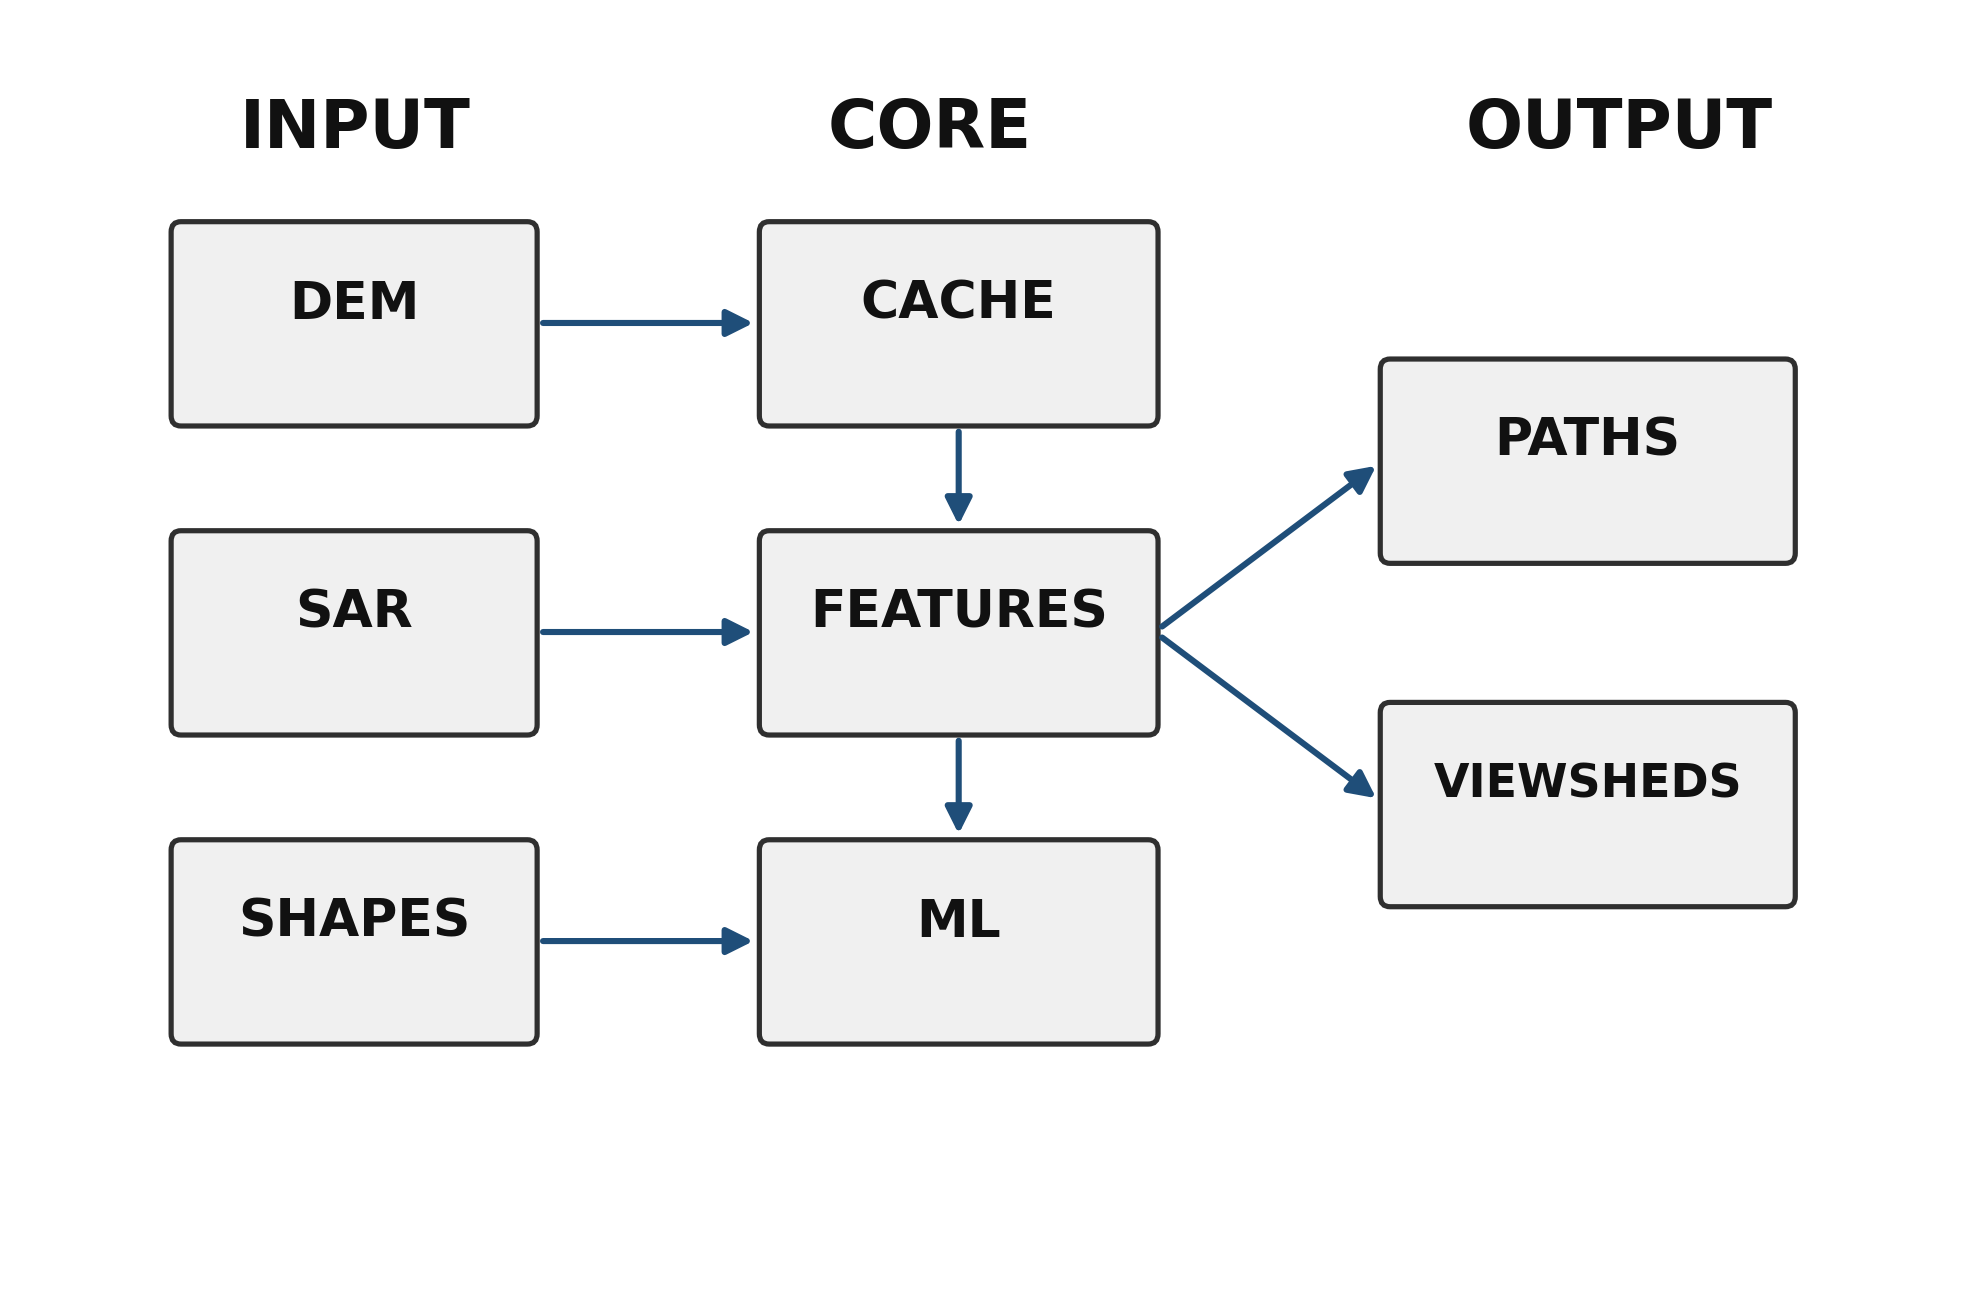
\includegraphics[width=\textwidth,height=0.54\textheight,keepaspectratio]{current_system.png}
    \caption{Current system view. Task outputs exist, but the validation layer is missing.}
\end{figure}

\clearpage

%----------------------------------
\section{Proposed Solution}

The proposal is simple: keep the existing LAMP tasks, add one alignment step between them, and add one comparison step after simulation.

Task 2 will export a visibility raster. That raster will be aligned to the Task 1 DEM grid. The aligned values will then act as one term in the cost model.

\[
C = w_s S + w_r R + w_t T + w_p (1 - P) + w_v (1 - V)
\]

Here, $V$ is visibility probability. When visibility is high, the penalty goes down. When visibility is low, the penalty goes up.

\begin{figure}[H]
    \centering
    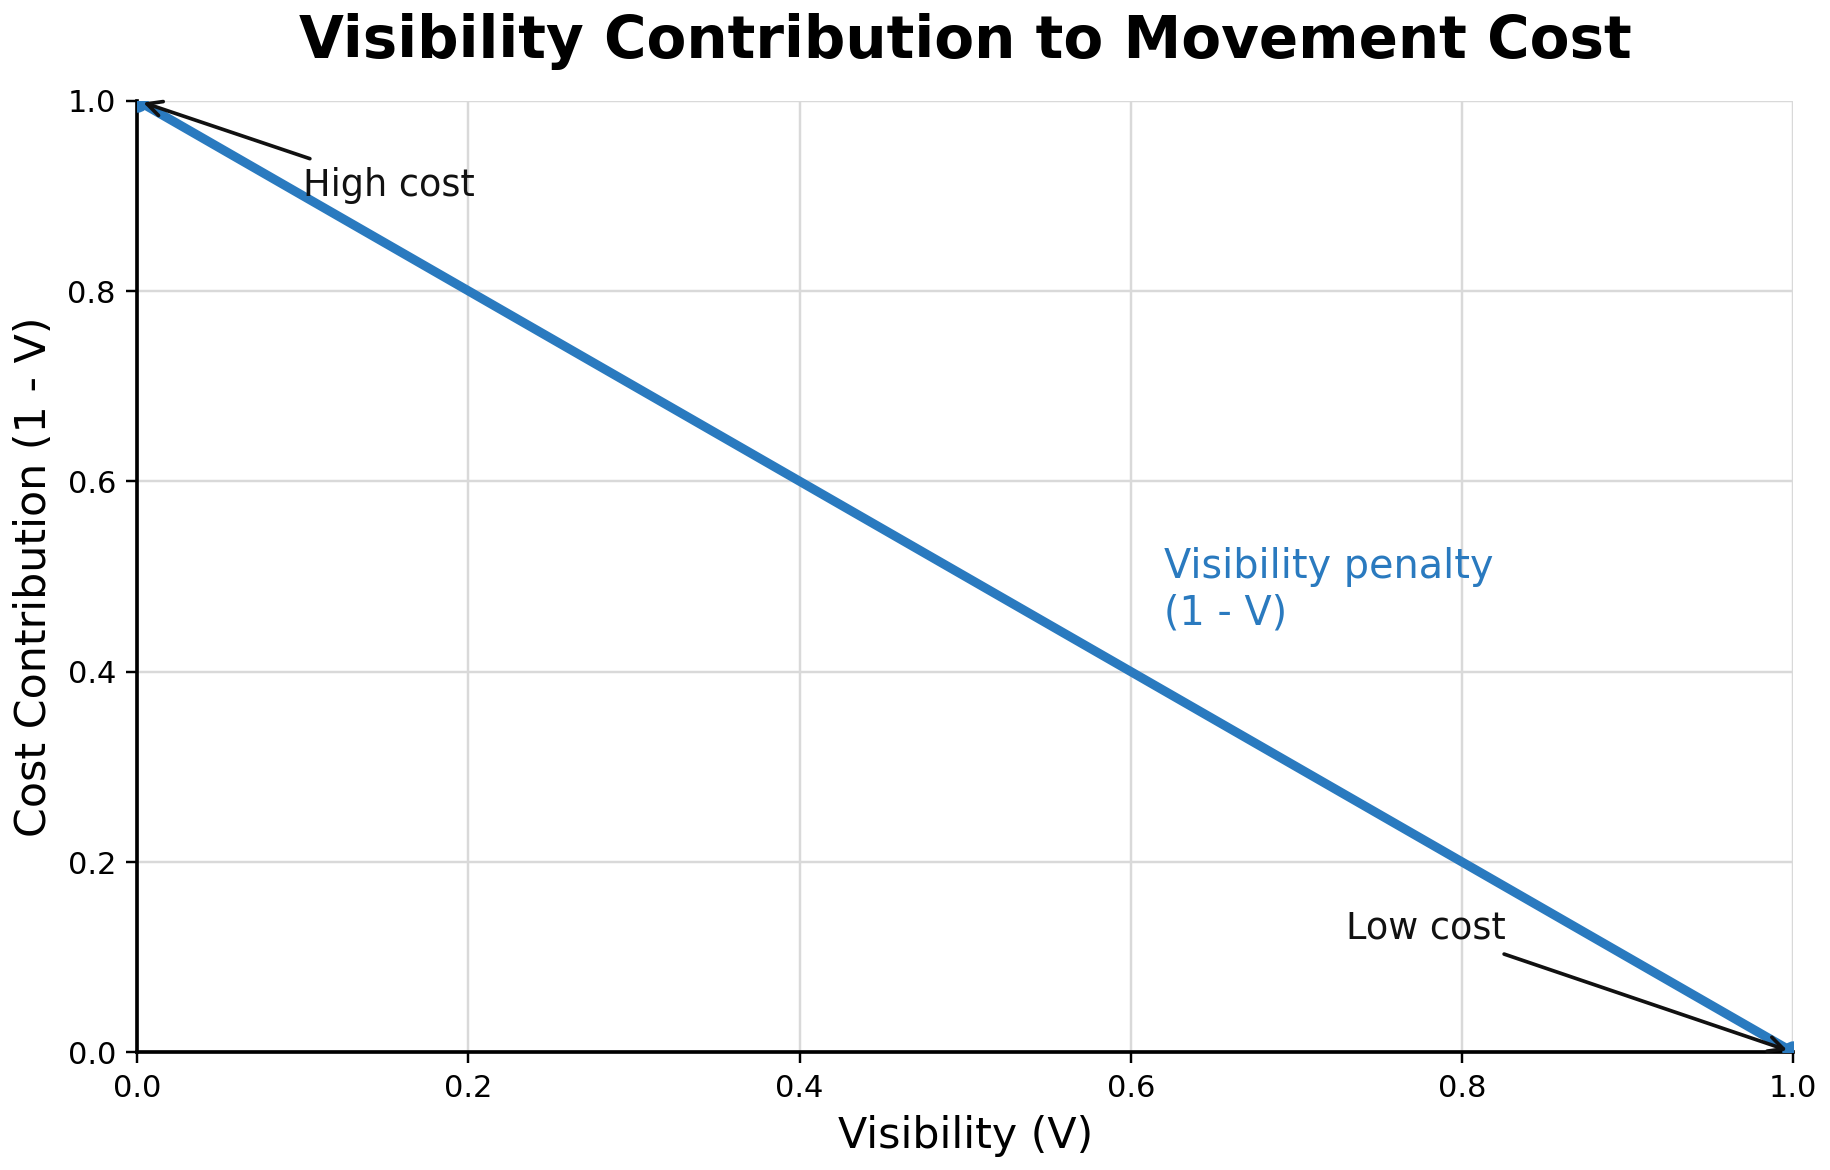
\includegraphics[width=0.86\textwidth]{cost.png}
    \caption{Visibility adds a simple linear penalty term to the movement cost.}
\end{figure}

\clearpage

%----------------------------------
\section{System Architecture}

The architecture stays close to the current repository design. The project does not need a new framework or a second pipeline. It needs a narrow interface between existing modules:

\begin{itemize}[leftmargin=1.4em]
    \item Task 2 visibility generation
    \item raster alignment and sanity checks
    \item Task 1 cost-surface construction
    \item path simulation
    \item comparison and metrics
\end{itemize}

Each stage writes files that can be inspected directly. That keeps the flow debuggable and reduces failure scope.

\begin{figure}[H]
    \centering
    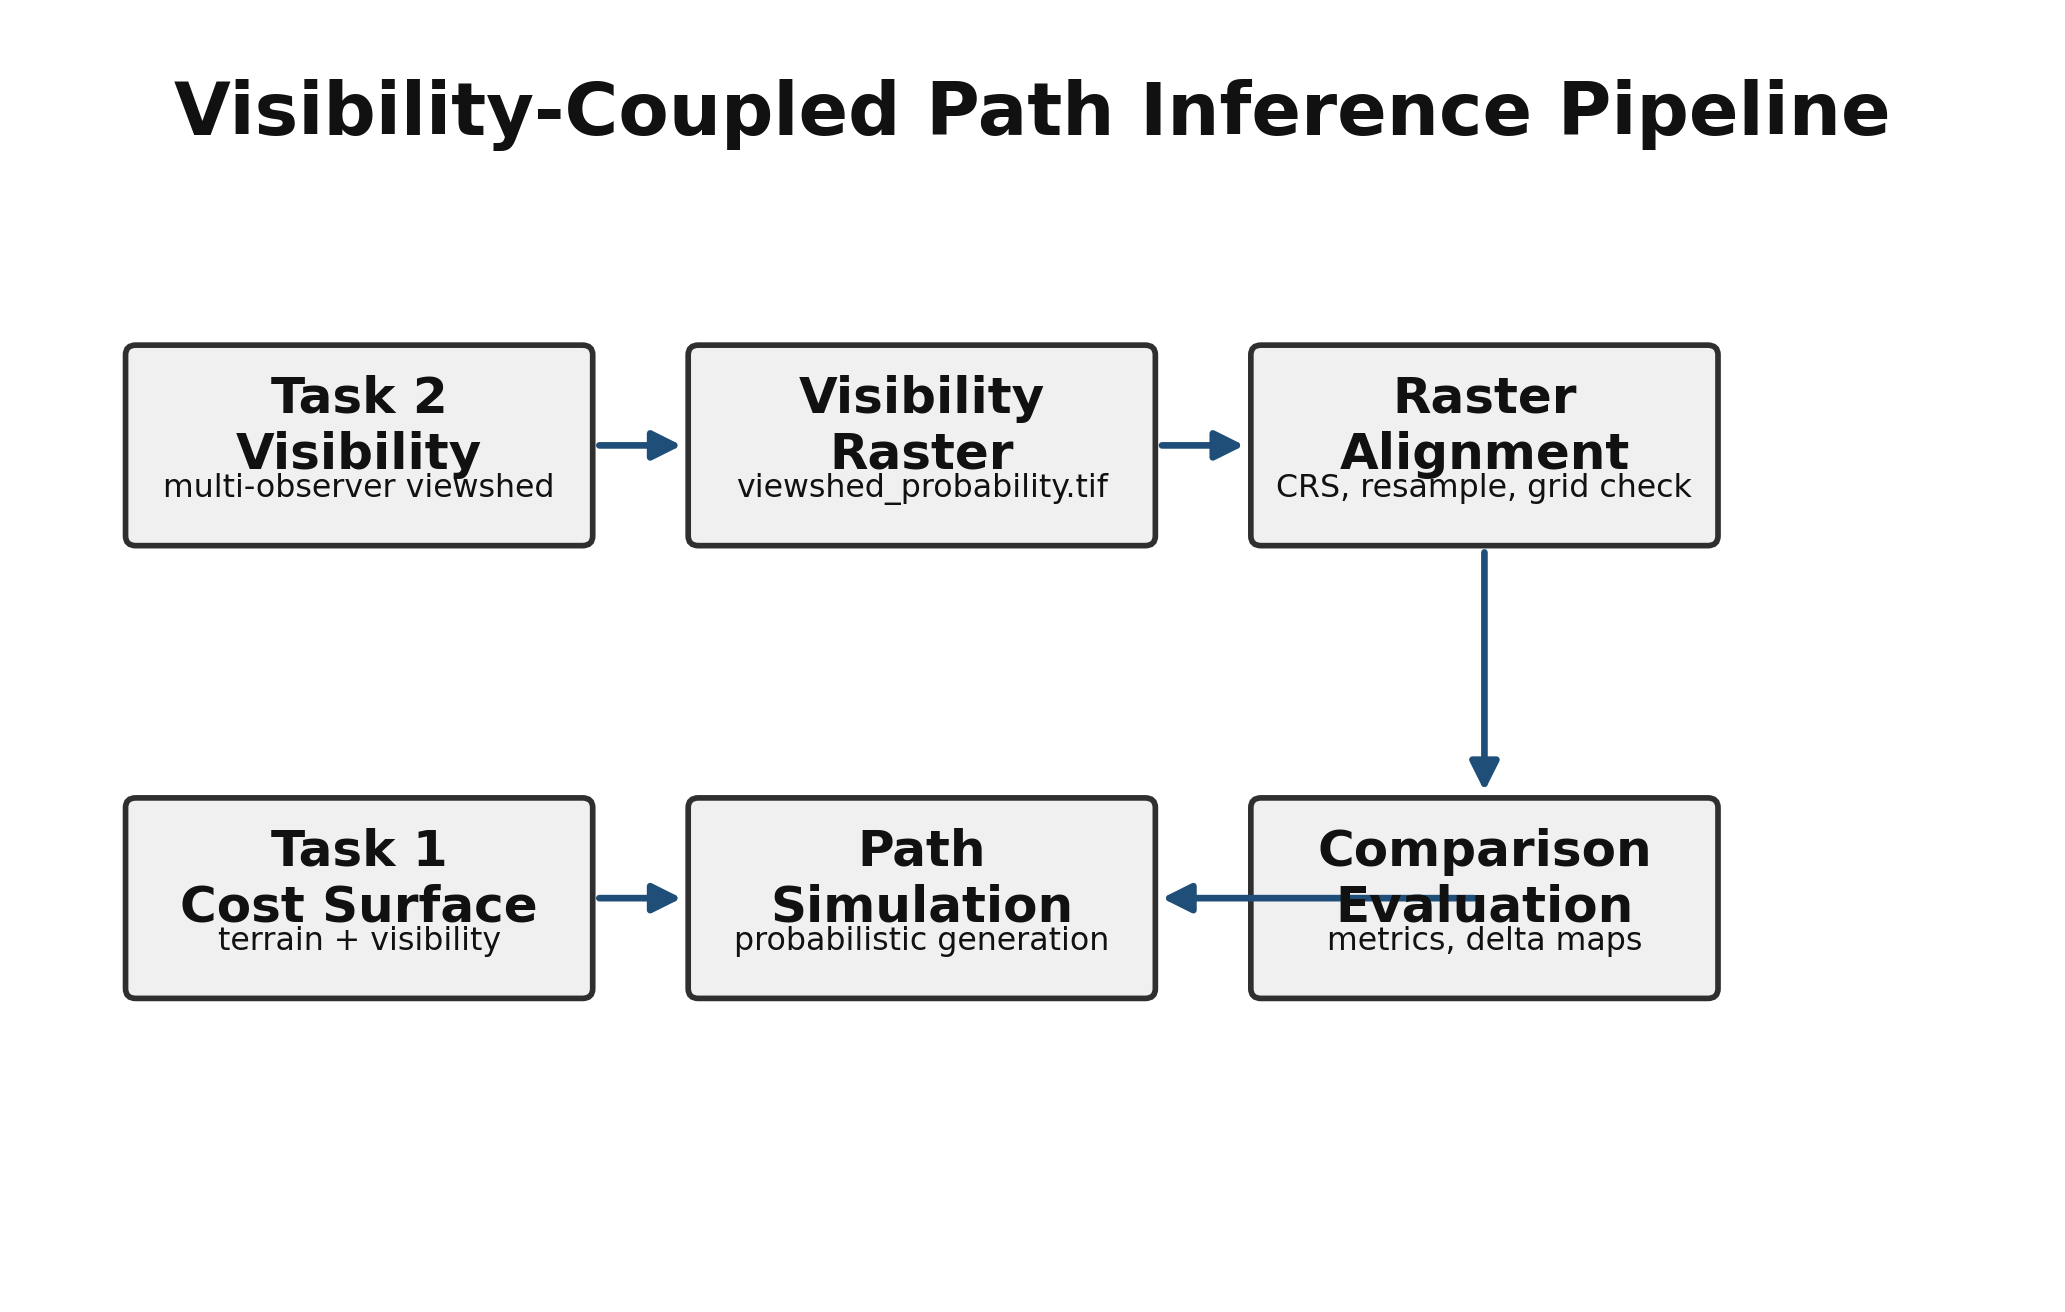
\includegraphics[width=\textwidth,height=0.64\textheight,keepaspectratio]{proposed_architecture.png}
    \caption{Proposed pipeline with visibility coupling and evaluation.}
\end{figure}

\clearpage

%----------------------------------
\section{Data Flow}

The data path is simple and deterministic:

\begin{verbatim}
DEM + buildings + observers
-> Task 2 viewshed computation
-> viewshed_probability.tif
-> CRS and grid alignment
-> Task 1 cost surface
-> path simulation
-> metrics and difference maps
\end{verbatim}

This flow matters because raster alignment is the main technical risk. If transforms, shapes, or CRS values do not match, the comparison is invalid even if the code runs.

\begin{figure}[H]
    \centering
    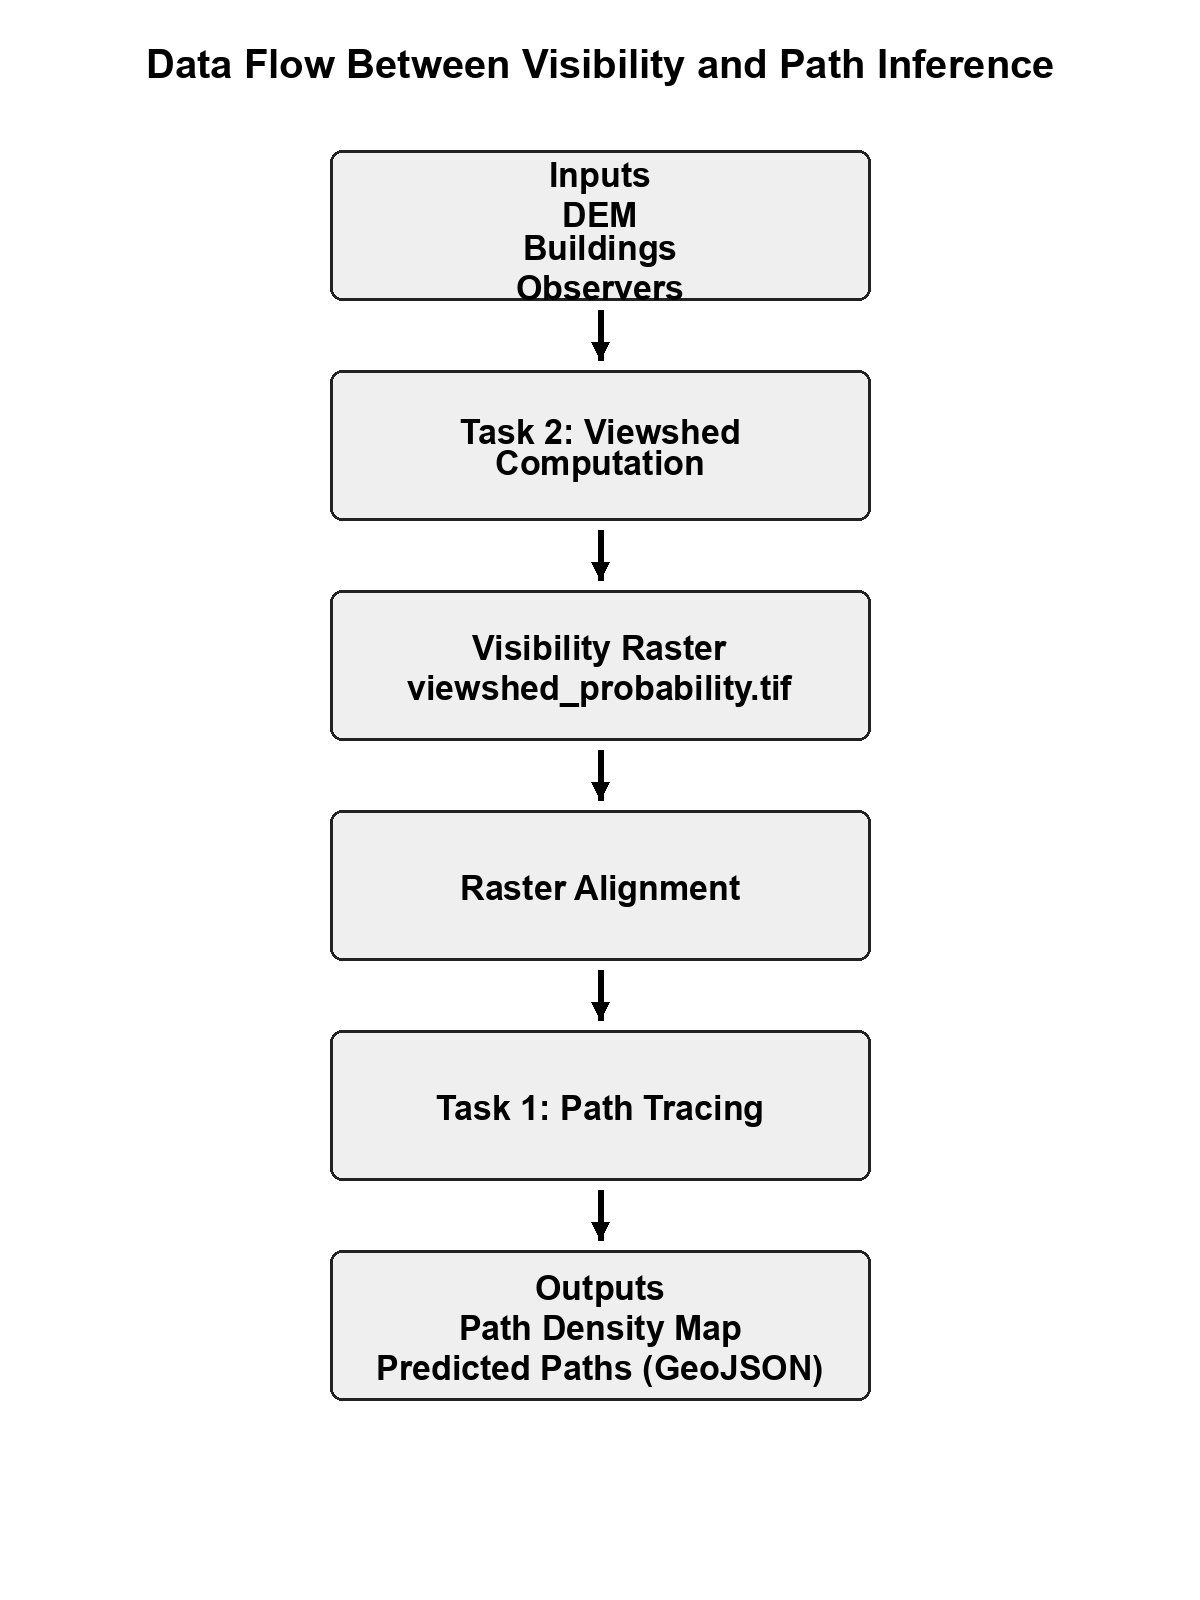
\includegraphics[width=0.88\textwidth,height=0.70\textheight,keepaspectratio]{dataflow.png}
    \caption{Data flow from inputs to final path comparison outputs.}
\end{figure}

\clearpage

%----------------------------------
\section{Detailed Design}

\textbf{Modules}

The work maps cleanly onto existing scripts and modules:

\begin{itemize}[leftmargin=1.4em]
    \item \texttt{scripts/run\_viewsheds.py}
    \item \texttt{scripts/run\_path\_tracing.py}
    \item \texttt{cost\_surface.py} for coupled cost construction
    \item \texttt{calibration.py} for bounded parameter search
    \item \texttt{visibility.py} for viewshed aggregation
\end{itemize}

\textbf{Core algorithm steps}

\begin{itemize}[leftmargin=1.4em]
    \item aggregate observer viewsheds into one probability raster
    \item check CRS, transform, and raster size
    \item resample when alignment fails
    \item run baseline and coupled simulations with the same seeds and inputs
    \item aggregate path densities and compute deltas
\end{itemize}

\begin{figure}[H]
    \centering
    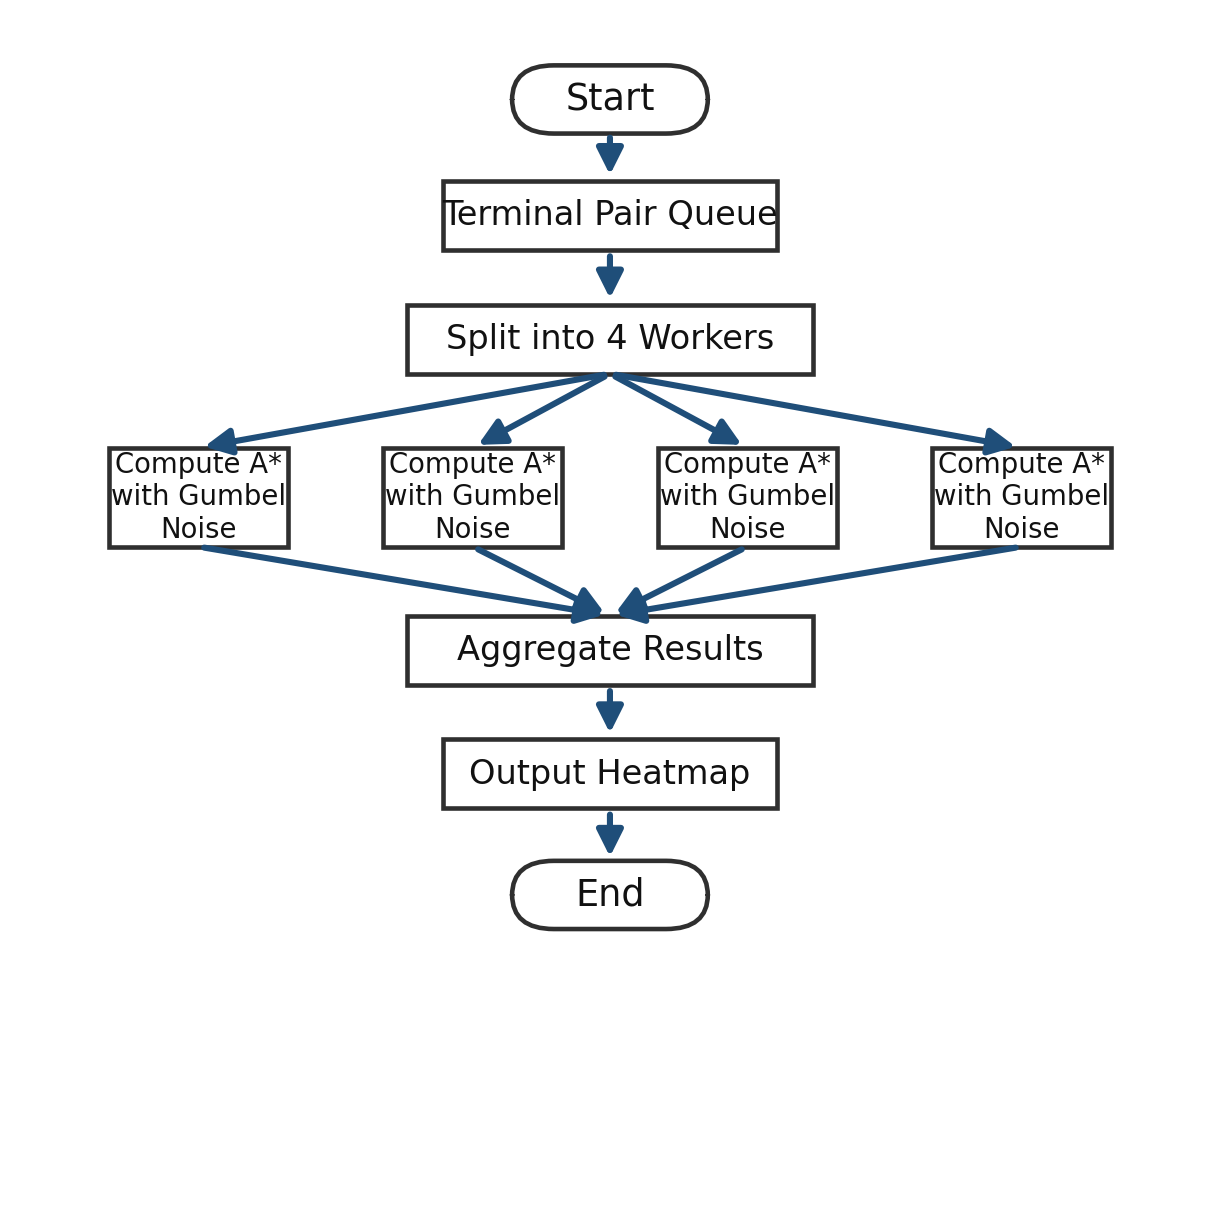
\includegraphics[width=0.72\textwidth,height=0.52\textheight,keepaspectratio]{modules.png}
    \caption{Module-level flow for path sampling and aggregation.}
\end{figure}

\clearpage

%----------------------------------
\section{Evaluation}

The project should produce evidence, not only output files. I will evaluate the coupled model in two ways.

\textbf{If archaeological ground truth is available:}

\begin{itemize}[leftmargin=1.4em]
    \item IoU
    \item F1 score
    \item top-k recall
\end{itemize}

\textbf{If ground truth is weak or missing:}

\begin{itemize}[leftmargin=1.4em]
    \item path-density divergence
    \item spatial redistribution analysis
    \item stability over a sweep of $w_v$
\end{itemize}

\begin{figure}[H]
    \centering
    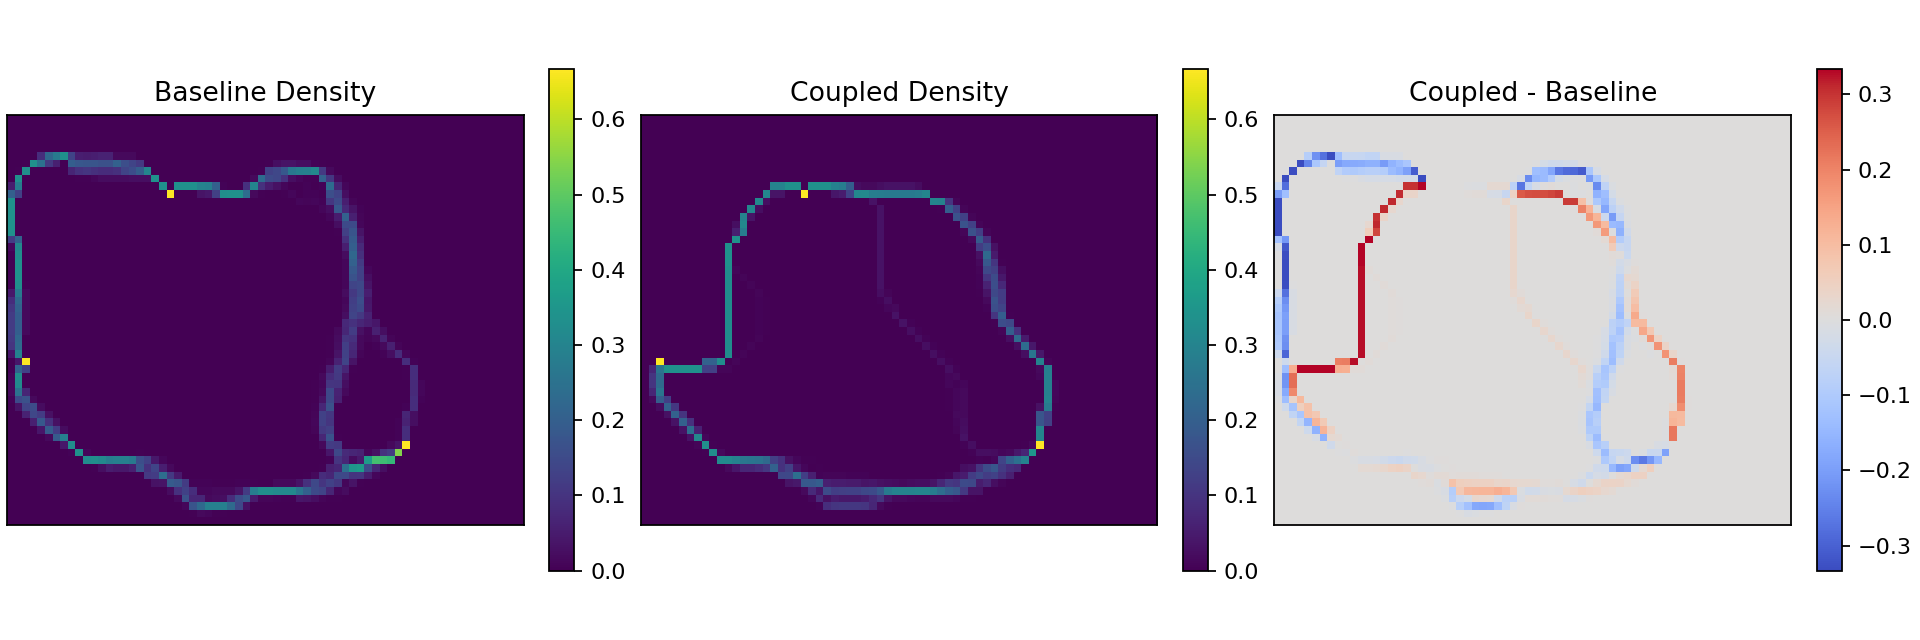
\includegraphics[width=\textwidth,height=0.54\textheight,keepaspectratio]{comparison.png}
    \caption{Baseline and visibility-aware path densities can be compared directly on the same grid.}
\end{figure}

\clearpage

%----------------------------------
\section{Difference Map}

The most useful visual output is the density delta map. It shows where visibility shifts movement probability, not just whether two runs are different.

This is the easiest way to inspect model behavior during calibration. If the coupled model only creates random noise, the difference map will show that quickly. If it redistributes movement in stable corridors, that is useful evidence even before formal scoring.

\begin{figure}[H]
    \centering
    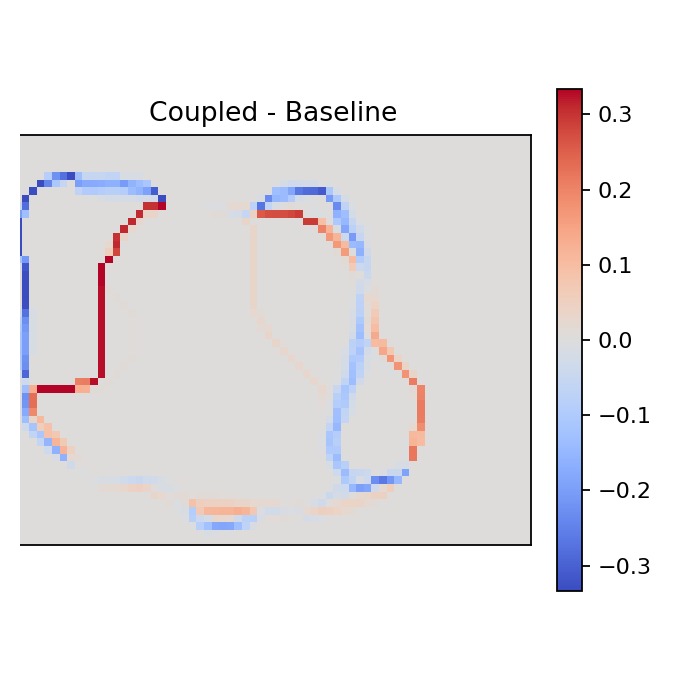
\includegraphics[width=0.78\textwidth,height=0.68\textheight,keepaspectratio]{difference.png}
    \caption{Difference map showing where visibility raises or lowers path density.}
\end{figure}

\clearpage

%----------------------------------
\section{Implementation Plan}

\begin{enumerate}[leftmargin=1.5em]
    \item Validate the baseline Task 1 run and record stable outputs.
    \item Run Task 2 and generate a real \texttt{viewshed\_probability.tif}.
    \item Align the visibility raster to the Task 1 grid.
    \item Inject visibility into the cost surface.
    \item Run baseline and coupled simulations under the same inputs.
    \item Sweep bounded values of $w_v$.
    \item Export metrics, GeoTIFF outputs, and vector artifacts.
\end{enumerate}

\section{Timeline}

\begin{tabular}{@{}lp{10.5cm}@{}}
\toprule
Weeks & Work \\
\midrule
1--2 & Environment check, dependency cleanup, baseline verification \\
3--4 & Task 2 execution and visibility raster export \\
5--6 & Raster alignment and cost-surface integration \\
7--8 & Baseline vs coupled simulation runs \\
9--10 & Calibration, metrics, and difference-map review \\
11--12 & Final write-up, artifacts, and reproducibility notes \\
\bottomrule
\end{tabular}

\clearpage

%----------------------------------
\section{Challenges and Risks}

\begin{itemize}[leftmargin=1.4em]
    \item GDAL or \texttt{osgeo} failures can block Task 2. I will resolve the runtime environment first.
    \item Raster misalignment can silently corrupt results. I will treat CRS, shape, and transform checks as hard gates.
    \item Ground-truth labels may be incomplete. In that case, I will rely more on density divergence and stable redistribution patterns.
    \item A weak visibility effect is still a useful result. It would show that visibility is not a strong constraint in the tested setting.
\end{itemize}

\section{Prior Work}

\begin{itemize}[leftmargin=1.4em]
    \item GitHub: \url{https://github.com/fallofpheonix}
    \item Prototype work on visibility-aware path modeling already exists, which lowers startup risk.
    \item My background fits the main tasks here: raster handling, simulation, and reproducible experiment design.
\end{itemize}

\section{Conclusion}

This proposal keeps the scope tight. It does not replace LAMP. It adds the missing validation layer that turns visibility coupling into something measurable, repeatable, and useful for archaeological interpretation.

\end{document}
